\chapter{Architecture/Model}
\label{cha:architectureAndModel}
This chapter contains the architecture and model of the system, which tools and methods that has been used, how they all connect together to run the experiments and produce the result.
An overview of the system is presented in chapter \ref{sec:overview}. A description of the robot is presented in section \ref{sec:robot}. Section \ref{sec:scenario} contains a description of the different scenarios used in the experiment.

\begin{figure}[h]
\begin{center}
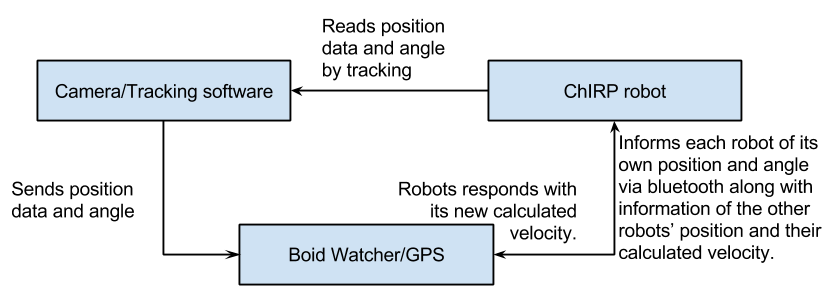
\includegraphics[width=\linewidth]{figs/system_overview}
\end{center}
\caption[System overview]{Overview of the components of the system}
\label{fig:overview}
\end{figure}

\section{System overview}
\label{sec:overview}

The system used in this experiment consists of three primary components as illustrated in figure \ref{fig:overview}: the camera which is used by tracking software, the "Boid-watcher" which is a centralized computer that acts as a GPS and the ChIRP robots.
The camera tracking software tracks each robot's position and its angle, which is sent to the Boid-watcher. The Boid-watcher then forward this information to the robots via the bluetooth serial port.

The Boid watcher does not only work as a GPS but it is also a bridge between the robots, it provides information about the position and velocity of each robot to all the other robots. The robots are not able to connect the other robots directly, that is why the robots need to pass information to other robots via the Boids watcher software.

Even if it is possible for one computer to run both the camera tracking and the watcher software, two separate computers were used in this setup. The camera tracking software being run on a stationary desktop computer, and the camera is attached to a pole above a sandbox where the robots roam around. The camera is connected to the stationary desktop. 

In this experiment, the watcher software runs on a laptop with built in bluetooth adapter. The watcher software needs to communicate with all the robots simultaneously and that requires a bit of processing powers.
The desktop computer was not able to run both the camera tracking software and the watcher software at the same time while sending bluetooth data to all four of the robots. When it tried to run both, it was not able to read the data from the camera fast enough and thus the tracking software would crash. The bluetooth connection between the computer and the robots might not always be stable, if the connection were to be unstable at times, a reboot of the robot or/and a reconnection of the bluetooth would usually fix the problem.

The camera tracks the robots using image recognition, it recognizes the robots by the two post it notes that are placed on top of each robot. 
To filter out all the noise from the surrounding and remove the colors that are irrelevant to track, the camera tracking software needs to have a threshold for what it considers to be red and what it considers to be green. This was specified in a configuration file that the camera tracking software loaded whenever it was launched. An example of the configuration file can be seen in the appendix on section \ref{app:opencvcfg}. As seen in the example, each color is defined by six boundaries, a minimum value and a maximum value. If a color seen by the camera is inside this boundary it will be considered as the color it is looking for. 

The camera might detect red or green colors that do not belong to the robot, for instance when the sun shines into the room, the green part of the floor around the sandbox might be detected as "green" by the camera tracking software. This is not a problem for the camera tracking software, the tracker only tracks inside a predefined box which the user has to specify when starting up the software as seen by the green outline in figure \ref{fig:camera}. Only the robots inside this predefined area will be tracked and have a legal position value associated with an angle, any robots found  outside of this green boundary box will have an undefined position. That is why we need a sandbox to contain the robots so they do not wander off outside the range of the green boundary box where they are not tracked anymore.

Detecting red or green color inside the sandbox that does not belong to the robots' post it notes imposes a bigger problem than detecting these colors outside the box. This might happen if there is a green shaded shadow or a reflection of an object inside the room reflects onto the sandboxes' surface. 
Detection of green or red color that do not belong to the robot is usually not a problem when the green and the red color are far apart from each other, because the camera tracking software does not do anything unless both these colors are paired. If these noise colors do disrupt the movement or angle of the robots, then a recalibration needs to be done to filter out the colors that it should not track.

\section{Robots}
\label{sec:robot}
\begin{figure}[H]
    \centering
    \begin{subfigure}[b]{0.3\textwidth}
        \centering
        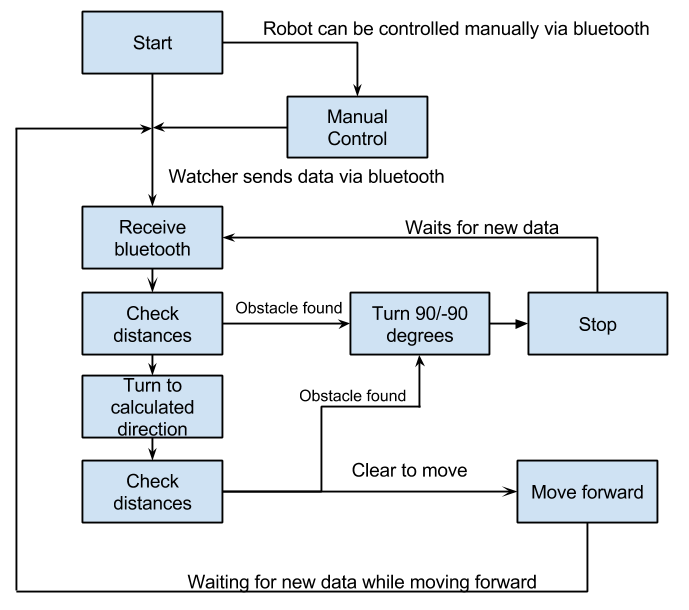
\includegraphics[width=\textwidth]{figs/robotschema.png}
        \caption{$y=x$}
        \label{fig:robot0}
    \end{subfigure}
    \hfill
    \begin{subfigure}[b]{0.3\textwidth}
        \centering
        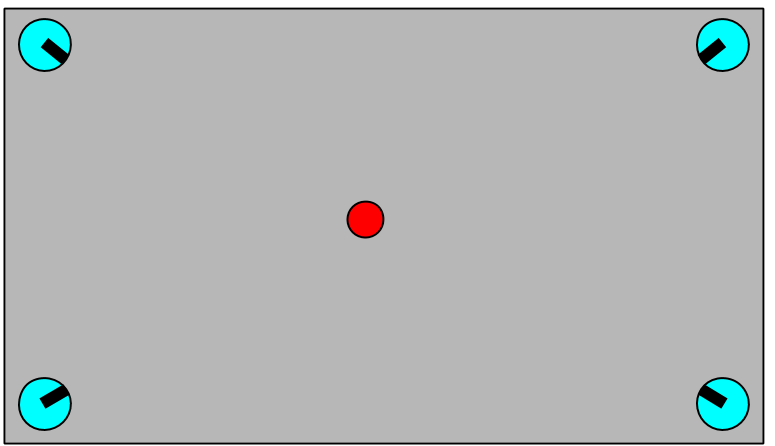
\includegraphics[width=\textwidth]{figs/scenario0.png}
        \caption{$y=3sinx$}
        \label{fig:robot1}
    \end{subfigure}
    \hfill
    \begin{subfigure}[b]{0.3\textwidth}
        \centering
        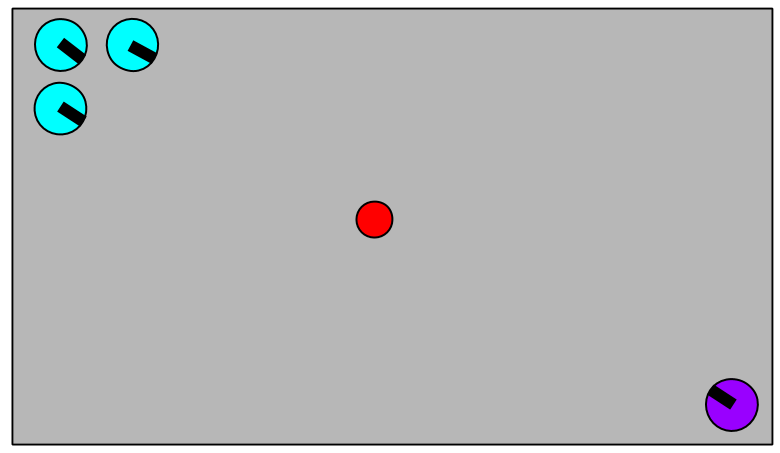
\includegraphics[width=\textwidth]{figs/scenario1.png}
        \caption{$y=5/x$}
        \label{fig:robot2}
    \end{subfigure}
    \caption[ChIRP robot]{ChIRP robot seen from various angles}
    \label{fig:robot}
\end{figure}


The robot swarm consist of four ChIRP robots. The ChIRP robot is a circular shaped robot with differential wheel. A differential wheeled robot is a robot with two separate driven wheels on each side, which it can use move itself. If it wants to change its direction it can vary the relative speed of each wheel/motor. For instance if the right wheel moves faster than the left one, the robot will turn to its left.
The advantage of differential wheel is that an additional steering motor is not required for the robot to move around. Usually a caster or additional wheels are added to balance a differential wheeled robot, but the ChIRP robot does not have anything of the sort. Whenever it is moving, the back or the front of the robot is scraping against the floor depending on which way it is moving. Scraping against the floor does not affect the movement of the ChIRP robot. The robots has a max speed of 13 cm/s, in this experiment the velocity of the robot will not exceed 7.8 cm/s. 

Each robot is equipped with eight infrared LED lights and receivers used for measuring distance. Infrared light are emitted the LED lights, reflected of a surface and received in the infrared receiver. For the robot to know how far from an obstacle it is, it measures the amount of infrared it receives. The higher the amount, the closer to the object it is. This method of measuring distances works very well for bright or colored surfaces, dark surfaces on the other hand do cause problems because the infrared light is not reflected so well.

The distance sensors are spaced evenly around the robot, where one of the sensors are directly in front of the robot. This sensor can be used to detect whether there is an obstacle directly in front of the robot or not. For this experiment, only the three sensors in front are used. Because the robots only moves forward, so it only needs to determine whether there is an obstacle directly in front of it or not. It does not matter if there is anything behind or next to the robot because it does not move in that direction.

Each of the ChIRP robot is equipped with a bluetooth module, which it uses to communicate with the watcher/GPS computer wirelessly. 
The robots are very hollow on top as seen in figure \ref{fig:robot}, and the distance sensors have difficulties sensing other robots due to the hollowness. To counteract the hollowness, a white paper strip was taped around the robots. This makes it easier for the robot to detect the other robots nearby because the paper will reflect the infrared light that the robot uses to determine the distance. To be sure that the robot would be able to detect the obstacles placed in the sandbox, the obstacle would have a white paper wrapped around it to reflect infrared light. The obstacle used for this experiment consist of bottle filled with water. The water inside the bottle is used to make the bottle heavier, so it does not fall over. And the paper around the bottle is there to reflect the infrared light that the robot uses for measuring distances.

The camera tracking software uses image recognition to track the robots. That is why each robot need to have a red and a green post it note on top of it. The red one determines where in the sandbox the robot is located, and the green one is used to determine which way it is pointing and to determine the angle of the robots.

\section{Scenarios}
This section explains the setup of each scenario, where each robot is placed in the sandbox, which way it is rotated and where the obstacle is placed. Each scenario have a purpose to demonstrate, which will be explained more in detail.
For this project experiment, three scenarios have been used to create the results seen in section \ref{sec:results}.
\label{sec:scenario}
\begin{figure}[h]
\begin{center}
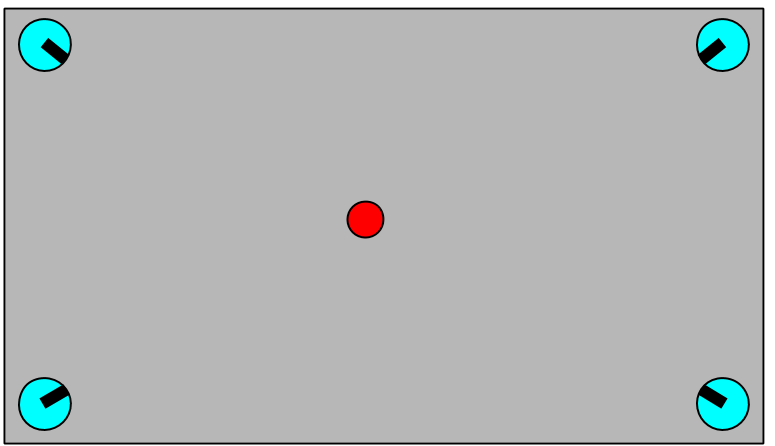
\includegraphics[width=0.8\linewidth]{figs/scenario0}
\end{center}
\caption[scenario 1]{Scenario 1, all the robots are placed in each corner with one obstacle}
\label{fig:scenario0}
\end{figure}

The first scenario is shown in figure \ref{fig:scenario0}, consists of four robots placed on each corner of the sandbox. The reason behind placing each of the robots on each corner of the sandbox is that each robot will be as far from each other as possible. This scenario should demonstrate that the entities are able to flock together, and then stay together as a flock. There is one obstacle placed nearby the middle of the sandbox, the obstacle is placed near the middle to ensure that the robots would encounter it at least once. This scenario would be able to see if the robots actually flocked together like they are supposed to do, and at the same time would be able to avoid the obstacle without bumping or crashing into it. The robots should also move together after they have flocked together.

\begin{figure}[h]
\begin{center}
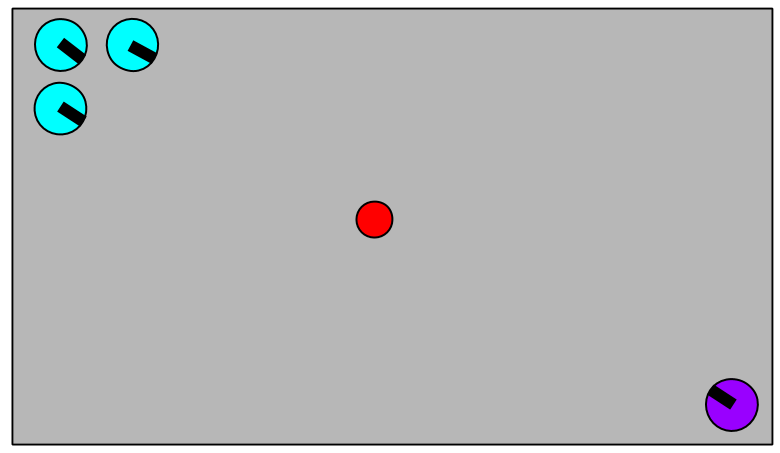
\includegraphics[width=0.8\linewidth]{figs/scenario1}
\end{center}
\caption[scenario 2]{Scenario 2, three robots in one corner, and the last one on the opposite corner}
\label{fig:scenario1}
\end{figure}

The second scenario puts three of entities in one corner, and the last entity is placed on the opposing corner as seen in figure \ref{fig:scenario1}. However the last entity that is placed on the lower right corner by itself will not move, in the case of the physical robot, it will not be turned on. The reason that this entity is a sitting duck placed on the opposite corner of all the other entities is that this robot will act as a goal for the other entities. The obstacle is placed between the lonely robot and the three robots that are clumped up together. The idea behind this setup is that the three robots that start together would try to move to the one that are stationary because they need to flock together. The robot that start by itself does not move because it is not turned on.
The obstacle in the middle will hinder the robots from moving in a straight line to their goal, which forces them to choose a way around it. The robots move around the obstacle when they approach it. As explained in section \ref{sec:robotArch}, the robots will turn either right or left randomly when moving directly towards an obstacle. The robots will probably move around the obstacle on each side of the obstacle, and flock together again on the other side when they have move past the obstacle.

The third scenario is a scenario where the robots are placed randomly around in the sandbox. The two first scenarios were designed for a specific purpose. The purpose of the third scenario is to demonstrate that the Boids behaviors are still intact, even when the robots are placed randomly in the sandbox. The position of the robots, where it should be placed and which way it is pointing was generated randomly by a random number generator. The starting point for this scenario is illustrated in figure \ref{fig:scenario2}. 

This scenario looks a little bit like the first scenario, the robots are laid out in the shape of a square. They are closer to each other than the robots in the first scenario. One of the robots are separated from the other by the obstacle, the robot can not move directly to the other three robots without moving around the obstacle.
\begin{figure}[h!]
\begin{center}
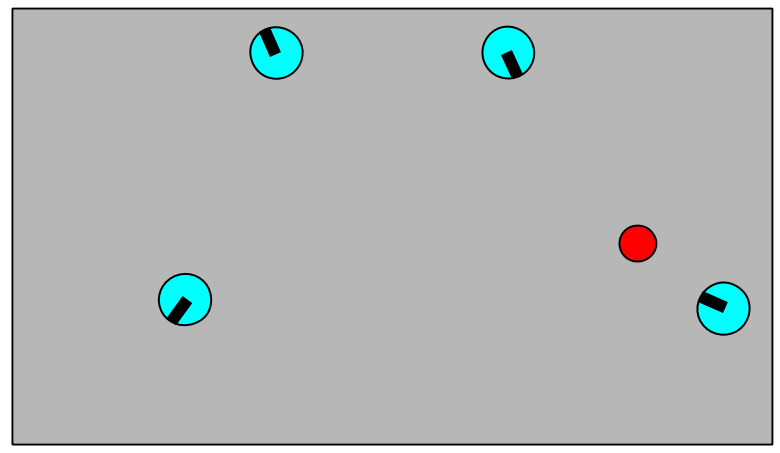
\includegraphics[width=0.8\linewidth]{figs/scenario2}
\end{center}
\caption[scenario 3]{Scenario 3, robots and obstacle randomly placed in the sandbox}
\label{fig:scenario2}
\end{figure}

All the scenarios explained in this thesis uses the same sandbox, which is a sandbox with the size of 151.6 cm wide and 123.9 cm long. The only difference between the scenarios are the placement and rotation of the robots and the placement of the obstacle. Each scenario were run ten times to generate the data seen in section \ref{sec:results}.
In between each run, the robots had to be placed manually back into their starting position before a new run could take place. To keep the data as consistent as possible, everything else would stay as exactly the same.

\section{Robot controller}
This section will go through the controller of the robot, how they work and what steps the robot takes to execute its action.

The robots is implemented using the idea of a hybrid robot control architecture as explained in section \ref{sec:hybrid}. The distances sensors are the reactive layers which will be used to guide the robots away from crashing into other robots, obstacle or walls. The deliberative layer will be the code that processes the data sent from the watcher software on the computer, it calculates where the robot should be heading. The executive layer would be the code running on the robot that decides what the robot is doing, whether that is reading the sensors and avoiding obstacles or towards the planned destination for flocking.

When the robot first is turned on and a bluetooth device is paired with its bluetooth module the robot will stand still and wait. The robot is waiting for a command or data from the watcher software. A human can send commands to manually control the robot if needed, this can be used for leader following as explained in section \ref{boids:behaviors}. 

If the watcher sends data to the robot, it will start to calculate where it should go based on the data it received. 
When the robot have received all the data it needs to be able to calculate its new direction that it should move to. The robot takes into consideration the position of all the other robots, and their velocity. The position of the other robots are used to determine the sum of the cohesion vector and the separation vector. The velocity of the other robots are used to determine which way they are pointing, and this is used to find the alignment vector. A fourth behavior was added for this experiment, which is called the "away from wall" behavior. As the name implies, this is a vector that will lead the robot away from the wall of the sandbox if the robot is too near the wall. After calculating each of these vectors, they are multiplied with a weight depending on how much that specific behavior should impact the movement of the robot. For example the separation vector should have higher impact on the movement of the robot because it needs to avoid the other robots when it is too close to one. Cohesion vector on the other hand does not need to affect the robot as much, it is mostly there to guide the robot into the flock. Therefore the separation vector is multiplied with a higher number than the other ones.

The equation for how the final vector which decides the direction the robot is going to move is expressed as:
\begin{equation}
\label{eq:vecsum}
\vec{F} = \Sigma W_x\vec{B_x}
\end{equation}

where:
\\
$\vec{F}$ = the final vector that determines which direction the robot will move
\\
$B_x$ = the behavior $x$, for example $B_0$ could be cohesion $B_1$ alignment etc.
\\
$W_x$ = the weight for the behavior $B_x$\\



When the robot has calculated which direction it wants to go, it will find out which direction it needs to face and turn itself approximately in that direction. The robot will then measure the distances once again, in case it has turned towards an obstacle. If there is no obstacle in front of it, it will move forward and wait for new data from the watcher software. If the robot did find an obstacle in front of it, it will turn 90\textdegree to either the right or the left randomly. The robot will stop after turning and wait for new data from the watcher software. 
\begin{figure}[h!]
\begin{center}
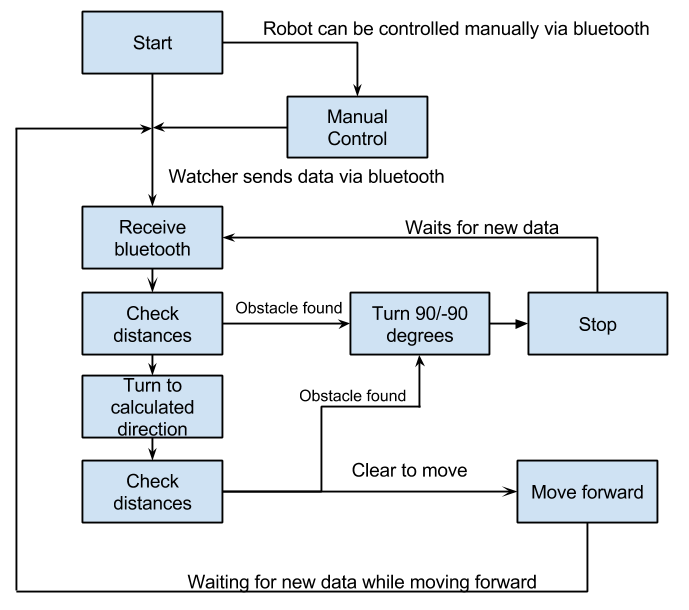
\includegraphics[width=0.8\linewidth]{figs/robotschema}
\end{center}
\caption[Robot flowchart]{Flowchart of the robot}
\label{fig:robotschema}
\end{figure}
\clearpage

\section{Simulator}
A simulator was created where the Boids was implemented solely in software, and rendered on screen, that is no physical robots were used in the simulator. The reason to use a simulator was to see how the Boids were supposed to behave and have a working example to compare with. A screenshot of the simulator is shown in figure \ref{fig:simulatordistances}.

A typical Boids simulator usually have a wraparound space. If one of the Boids goes outside the window, it will "teleport" to the other side of the window. For example if one of the Boids flies too far to the right and hits the right border, it will loop around and end up on the left side of the screen. That is how the Boids algorithm usually works on a simulator. But physical robots can not loop around the stage like the Boids on the simulator. That is why the simulator used in this project stops the Boids from moving beyond the walls of the window.

The same "away from wall" behavior is also implemented in the simulator, so the Boids do not move into the wall aimlessly.
For each frame, the Boids will update it velocity by calculating a vector for each behavior, and then these vectors are added to the acceleration vector by using the formula found in equation \ref{eq:vecsum}. The acceleration vector is then added to the velocity vector, and the velocity is capped off if the length of the vector exceeds maximum allowed speed. If there is no velocity cap, the Boids' velocity would increase towards infinity. The velocity then decides where the Boids are going to move.
Before the next time step, the acceleration has to be reset to a null vector for it to work.

The Boids in the simulator does not have any form of rotation, the angle seen on screen are calculated by taking the arctangent of the velocity vector. That is why the Boids in the simulator do not need to rotate; they rotate instantly by changing their velocity.

In the simulator, there is no need for any type of sensors. Each Boid have access to the location of all the obstacles and all the other entities.

Each Boids in the simulator are circular, so they are as similar as the real ChIRP bot, however there is some big differences between the real ChIRP robot and the Boids in the simulator.

\section{Differences between the physical experiment and simulator}
The physical robots are trying to mimic the behavior of the Boids created in the simulator. However a physical robot is different than the Boids created in the simulator by nature. As discussed in section \ref{sec:robot}, the robots are a type of differential wheeled robots, which means that it can only move forward or backwards, turn on the spot or move and turn at the same time. It can not move sideways.

The Boids in simulator software did not have any direction, they were able to move freely in all 360\textdegree direction. Which means that if a Boid in simulator were to move in one direction, it could change its momentum and move the other direct without having to stop and turn to that direction. The robot on the other hand would need to turn 180\textdegree before moving forward. The robot is able to reverse its motor to drive backwards, but these Boids robot are not allowed to move backward, and thus have to turn around to move in another direction.

In the simulator, each Boid will know exactly where everything is placed. That is, each Boid knows where all the other Boids are, including itself. It also knows where all the obstacles are. The Boids will have real time access to everything that can be seen on screen. Every Boids will update its perception every frame, that is approximately 60 times every second.

The robots on the other hand, will receive data from the watcher about all the other robots. But due to inaccuracies from the camera and the image processed, the robots only knows vaguely where in the sandbox it is located, and where the others are. The time it takes for a robot to receive new information from the watcher takes roughly one second from the last time it received data from the watcher. If the robots are moving between the time it receives data, it will not know where it is before it receives new data from the watcher software. The camera tracking software are able to see all the robots due to the two post it notes on top, but obstacles found in the sandbox do not contain any color or anything that the camera can track. Obstacles are therefore ignored by the camera tracker software because it does not support tracking of anything other than the robots. That is why the robots needs to use their distance sensors in front to detect the obstacles.

The biggest most visual difference between the physical experiment in the sandbox and the simulated Boids is the size and speed of the entities. The size of the simulator is 1024 px times 1024 px. While the sandbox is 151.6 cm wide and 123.9 cm long, which corresponds to 800x652 px in the watcher software. The Boids on the simulator moves quite fast and can use the extra space to move around, while the robots are confined inside the sandbox. The biggest reason to use 800x652 px for the watcher software is because the behavior neighborhood distances works well for this size.

\begin{figure}[h]
\begin{center}
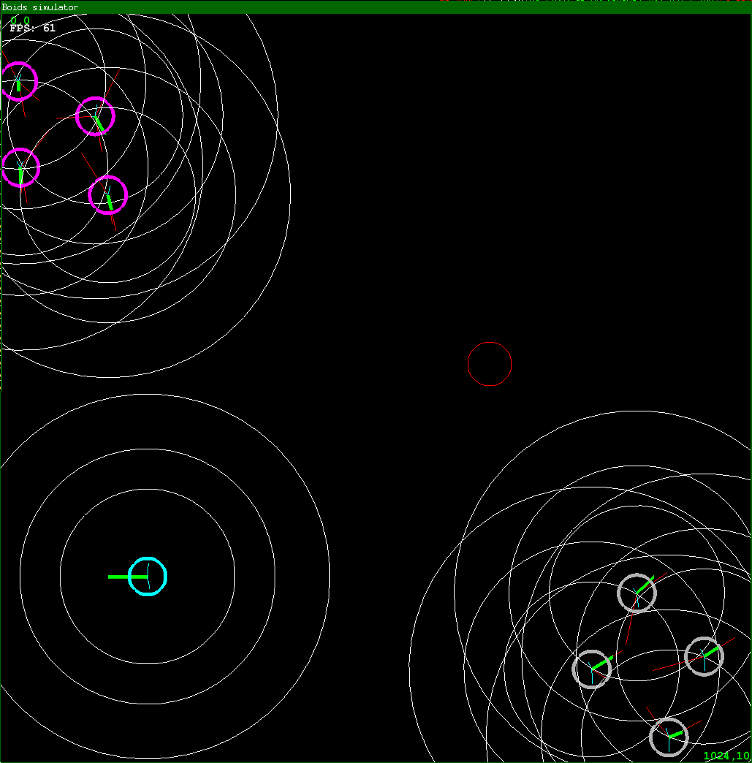
\includegraphics[width=0.8\linewidth]{figs/simulator}
\end{center}
\caption[Simulator distances]{Boids with neighborhood distances visualized}
\label{fig:simulatordistances}
\end{figure}

As it will be explained later in section \ref{sec:experimentalSetup}, the parameters for the simulated Boids and the physical robots are a bit different.
The figure \ref{fig:simulatordistances} shows the approximate distances for each behavior, the inner thick colored ring is the outline of the Boids. The inner thin white ring, illustrates the separation distance, the robot do not try to separate itself from the other robots when they are outside this ring.

The red lines in the figure, is the vectors from each behavior before it is multiplied with the weight. The thickest green line indicates which way the Boids are facing.

The second most outer ring indicates the alignment neighborhood, all there is another robot inside this ring, the robot will try to point in the same direction so they move together in the same direction.

The outer circle is the cohesion distance, the Boids outside of this box will not attract each other.


In the figure \ref{fig:simulatordistances}, three types of Boids exist, each one have their own color. Boids will flock together and align themselves only if they have the same color, that is the light gray Boids will flock together with the other light gray Boids. The magenta Boids will only flock together with the other magenta Boids.
When running the simulation for the experiment, all four of the Boids were the same color, therefore just one flock of Boids would emerge instead of forming multiple flocks. The current implementation of the Boids algorithm on the robots do not support multiple groups of Boids. There is no point in implementing this functionality when there are only four robots running at the same time, because it will be very hard to distinguish the difference between a family group flock or if there is just a robot astray from the flock.

\begin{figure}[h]
\begin{center}
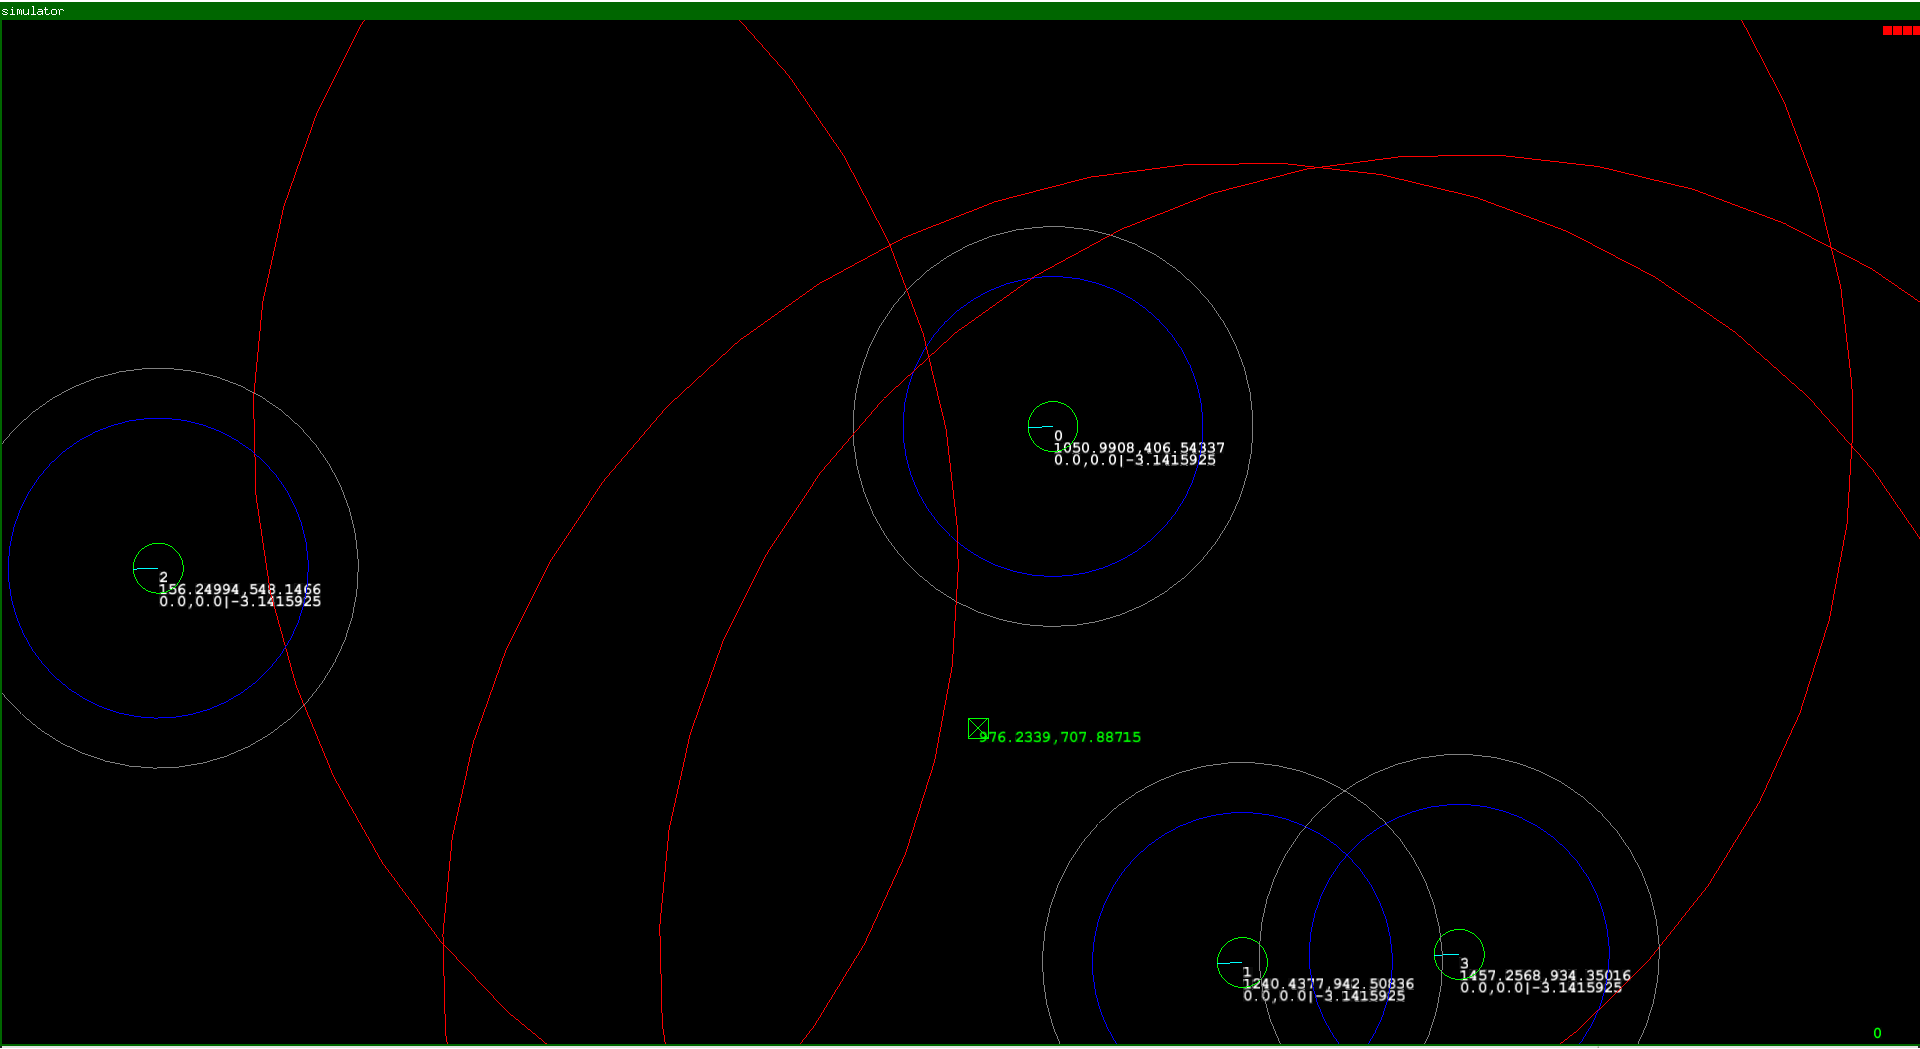
\includegraphics[width=1.1\linewidth]{figs/wathcer}
\end{center}
\caption[Watcher software]{Watcher software with neighborhood distances visualized}
\label{fig:watcher}
\end{figure}

Figure \ref{fig:watcher} illustrates the distances that the robots uses. The exact numbers can be found in section \ref{sec:experimentalSetup}. The distances have been colored for convenience, because it is hard to see which ring represents which behavior. As in the simulator, the most inner ring, which is green in this figure represents the outline of the robot. The figure shown is not the same size as the watcher software that is used to run the experiments, the resolution of the watcher software on the figure has a resolution of 1024x1920 px which is a lot bigger than the resolution on the watcher software used in the experiment. This is to make it easier to see and distinguish the distances.

The next ring, which is illustrated with a blue color, represents the separation distance. And the gray ring shows the alignment neighborhood distance. These two distances are the same in the simulator and on the robot.

The biggest red ring is the one that is the most different from the simulator's. The ring is quite big. The robots might get stuck in a corner, or drive around in circles.
The reason the cohesion distance is so large is mainly to force the robots to flock together even when their are far apart. The distance almost covers the whole sandbox, that way the robots will try to flock from almost anywhere in the sandbox.

Information about each robot is also provided by the numbers next to each robot.
The first row show us the ID of the robot, and the serial port that belongs to that robot if there is a bluetooth connection and it is assigned.
Second row shows us the position of the robot, while the third one shows velocity and the angle of the robot.

The uppermost red squares indicates whether the bluetooth connection is still functional or if the bluetooth have timed out. The squares in the figure are all red, because this is just a debug run where there is no bluetooth connection.